\documentclass[10pt]{beamer}
%\usepackage[spanish]{babel}
%\selectlanguage{spanish} 
\usepackage[utf8]{inputenc}
\usepackage{default}
\usetheme{Montpellier}
%\usecolortheme{dolphin}
\usecolortheme{whale}
\usepackage{graphicx}
\usepackage{float} % supuestamente sirve para las tablas, con [H] se ponen en donde uno quiere
\restylefloat{table} % supuestamente sirve para las tablas, con [H] se ponen en donde uno quiere

\usepackage{subfig}    %para hacer figuras multiples
%\usepackage{hyperref}
\usepackage{cancel}

\begin{document}

\title[The TOROS collaboration]
{TOROS: The O1 Advanced LIGO science run}

\institute{IATE - CONICET - (UNC)\\ University of Texas at Rio Grande Valley \\ Texas A\&M University}
\titlegraphic{
\includegraphics[scale=0.8]{./slides/plots/vitraux_h90.png}}
\author{
\begin{tabular}{r@{ }l} 
Author: Diego G. Lambas, & Bruno S\'anchez,   & Mariano Dom\'{i}nguez,  & Marcelo Lares, 
        & Mario D\'{i}az,  & Mart\'{i}n Beroiz,  & Tania Pe\~nuela, & Lucas Macri, & Carlos Colazo & \& Many more
\end{tabular}}

\frame{\titlepage}
\begin{frame}
\frametitle{Contents}
\tableofcontents%[sectionstyle=show/hide, 
    %sectionstyle=show/shaded]
\end{frame}


\section{Gravitational Waves detected in 2015}
%%%%%%%%%%%%%%%%%%%%%%%%%%%%%%%%%%%%%%%%%%%%%%%%%%%%%%%%%%%%%%%
%%%%%%%%%%%%%%%%%%%%%%%%%%%%%%%%%%%%%%%%%%%%%%%%%%%%%%%%%%%%%%%
%%%%%%%%%%%%%%%%%%%%%%%%%%%%%%%%%%%%%%%%%%%%%%%%%%%%%%%%%%%%%%%
\begin{frame}
LIGO Gravitational Wave observatory scientific run O1 
spanned September trough January 2016.

It produced two positive detections of GW events.
\begin{figure}%[h]
 \centering
 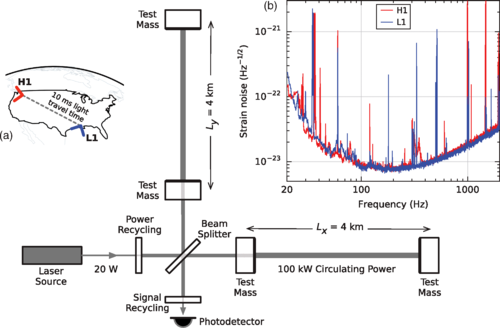
\includegraphics[width=0.65\textwidth]{./slides/plots/medium.png}
 \caption{\scriptsize{The detector configuration. }} 
\end{figure}
\end{frame}
%%%%%%%%%%%%%%%%%%%%%%%%%%%%%%%%%%%%%%%%%%%%%%%%%%%%%%%%%%%%%%%
\begin{frame}
There was a positive detection in September 14 of 2015, 4 days
before LIGO O1 scheduled observations start, with an estimated
S/N ratio of almost 24.

The pipeline final calibration for event detection was completed 
just 2 days before cWB pipeline reported a candidate.

\begin{figure}%[h]
 \centering
 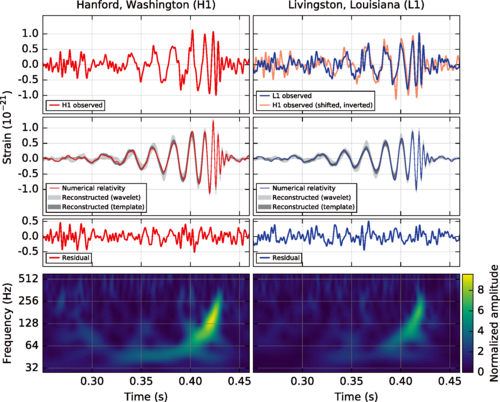
\includegraphics[width=0.6\textwidth]{./slides/plots/medium_fp.png}
 \caption{\scriptsize{Pipeline results, for matched filter techniques.}} 
 
\end{figure}
\end{frame}
%%%%%%%%%%%%%%%%%%%%%%%%%%%%%%%%%%%%%%%%%%%%%%%%%%%%%%%%%%%%%%%
\begin{frame}
The candidate was estimated to come from a huge area in the sky.
\begin{figure}
 \centering
 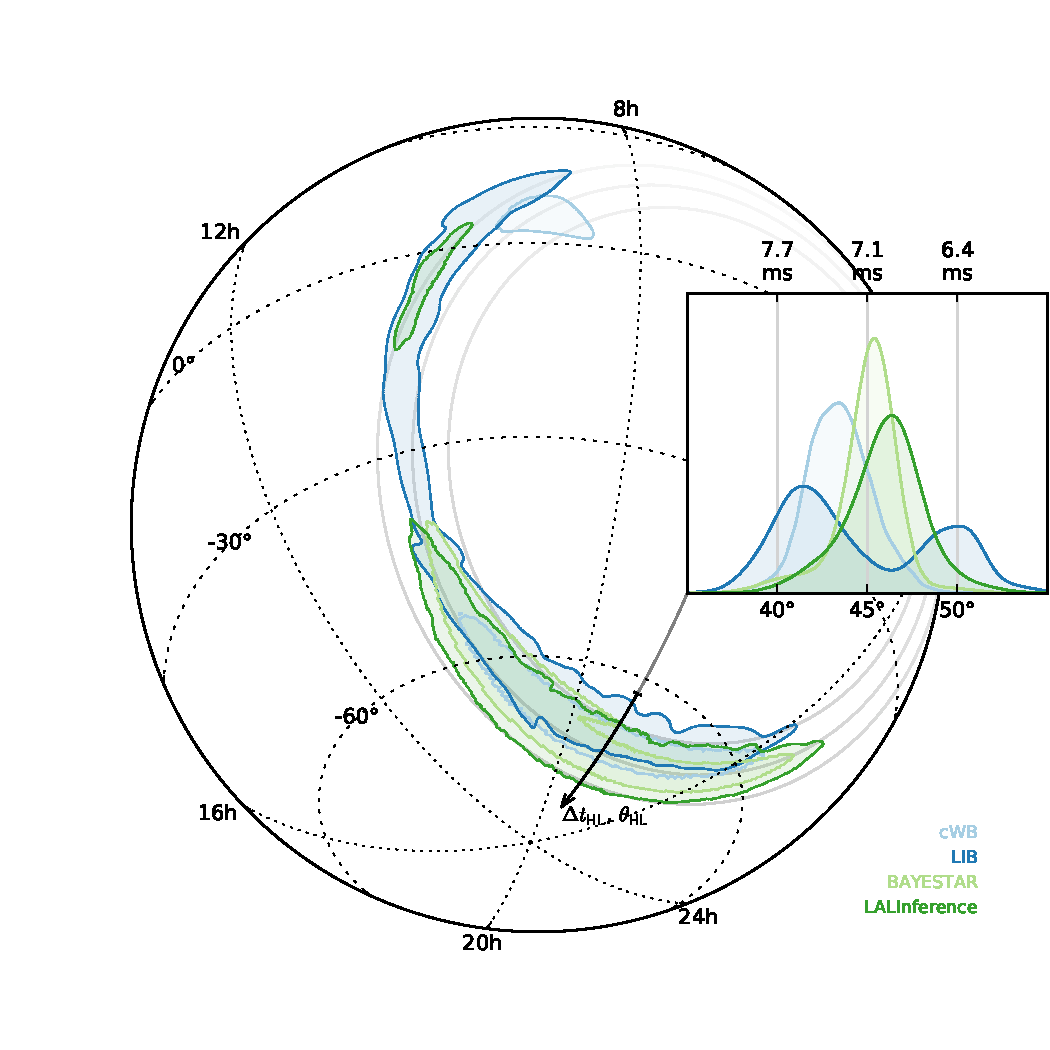
\includegraphics[width=0.8\textwidth]{./slides/plots/160208492v4/contours.pdf}
 
 \caption{Contours of sky localization}
 \label{fig:contours}
\end{figure}
\end{frame}
%%%%%%%%%%%%%%%%%%%%%%%%%%%%%%%%%%%%%%%%%%%%%%%%%%%%%%%%%%%%%%%
\begin{frame}
There are several pipelines for different purposes:

\begin{itemize}%[<+->]
 \item[cWB] Means coherent Wave Burst, and searches for unmodeled bursts
 of energy in the power-time-frequency space. Mostly based on antenna pattern, 
 and minimal assumptions of waveform morphology.
 
 \item[oLIB] Stands for omicron+LALinference Burst. Also searches for 
 bursts that are not modeled as a binary. LIB works assuming that the 
 signal is a sinusoidally modulated Gaussian, this pipeline performs 
 sky localization bayesian inference.
 
 \item[Bayestar] This method triangulates the times, the phases, and the 
 amplitudes of the signal arrival in both detectors.
 
 \item[LALinf.] This pipeline uses Compact Binary Coalescence (CBC) 
 template matching, by modelling the data with a parametrized CBC waveform.
 This is the most accurate pipeline, but it takes longer to compute
 due to high dimensionality.
\end{itemize}

\end{frame}
%%%%%%%%%%%%%%%%%%%%%%%%%%%%%%%%%%%%%%%%%%%%%%%%%%%%%%%%%%%%%%%
\begin{frame}
The full area of the 90\% confidence in the final LALinference map, 
which could be shared almost 2 days after detection, is $630 \ deg^2$\\
%\pause
At this time there was no information about the true nature of the source.
And the scenario was urging for more data, specially electromagnetic (EM)
follow up.\\

\begin{figure}
 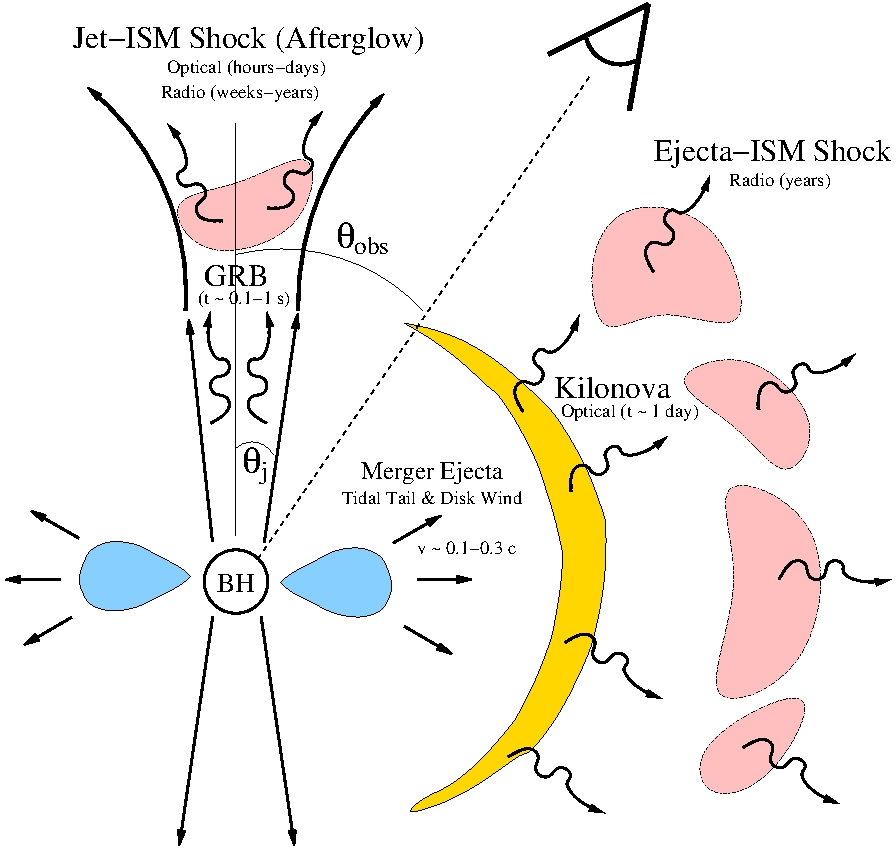
\includegraphics[width=0.45\textwidth]{./slides/plots/cartoon.jpg}
 \caption{\scriptsize{Compact object merger cartoon}}
\end{figure}
\end{frame}
%%%%%%%%%%%%%%%%%%%%%%%%%%%%%%%%%%%%%%%%%%%%%%%%%%%%%%%%%%%%%%%
\section{TOROS/TORITOS}
%%%%%%%%%%%%%%%%%%%%%%%%%%%%%%%%%%%%%%%%%%%%%%%%%%%%%%%%%%%%%%%
%%%%%%%%%%%%%%%%%%%%%%%%%%%%%%%%%%%%%%%%%%%%%%%%%%%%%%%%%%%%%%%
\begin{frame}
\textit{Transient Optical Robotic Observatory of the South}

The project TOROS, and its pilot campaings named 
TORITOS, are a collaboration for the installation of optical
telescopes at the Puna montains in Salta, at nearly 4600 m.

This places have really great atmospheric conditions for astronomy, 
and a high percentage of clear nights.

\begin{figure}
 \centering
 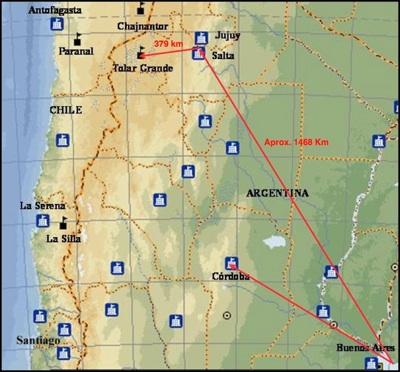
\includegraphics[bb=0 0 400 372, width=0.3\textwidth]{./slides/plots/Site.jpg}
 % Site.jpg: 400x372 pixel, 72dpi, 14.11x13.12 cm, bb=0 0 400 372
 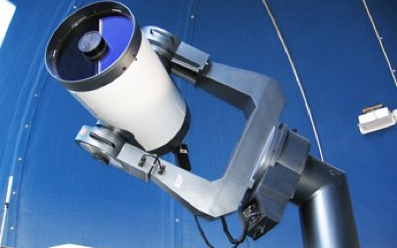
\includegraphics[bb=0 0 159 99, width=0.45\textwidth]{./slides/plots/toritos_1.png}
 % toritos_1.png: 397x248 pixel, 180dpi, 5.60x3.50 cm, bb=0 0 159 99
\end{figure}
\end{frame}
%%%%%%%%%%%%%%%%%%%%%%%%%%%%%%%%%%%%%%%%%%%%%%%%%%%%%%%%%%%%%%%
\begin{frame}
 The collaboration participated in the EM searches of GW150914.
 \begin{figure}
 \centering
 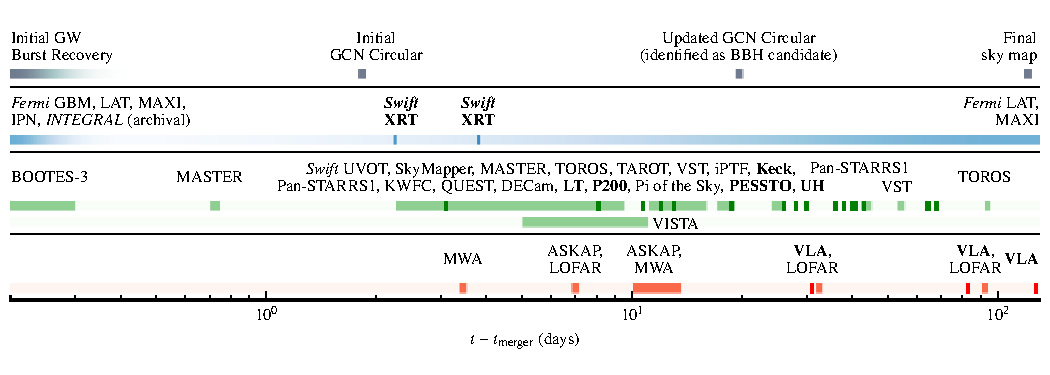
\includegraphics[width=\textwidth]{./slides/plots/160208492v4/timeline.pdf}
 % timeline.pdf: 0x0 pixel, 300dpi, 0.00x0.00 cm, bb=
 \caption{Timeline of detection}
 \label{fig:timeline}
\end{figure}
\end{frame}
%%%%%%%%%%%%%%%%%%%%%%%%%%%%%%%%%%%%%%%%%%%%%%%%%%%%%%%%%%%%%%%
\section{The TOROS observation method}
\begin{frame}
There are several collaborations that signed a Memorandum of Understanding
which stated the sharing policies for transient search.\\
%\pause
Some of them perform wide area blind search, with many telescopes, surveying the 
area of Likelihood from sky maps.\\
%\pause
TOROS collaboration performed a different search method, by crossmatching 
catalogs of galaxies from White et al. (2011) with the Likelihood map. 
This is due to small Field of View of telescopes.\\
\end{frame}
%%%%%%%%%%%%%%%%%%%%%%%%%%%%%%%%%%%%%%%%%%%%%%%%%%%%%%%%%%%%%%%
\begin{frame}
 We selected galaxies that had both high likelihood ratio, and as 
 at the time the sensitivity of A-LIGO (in engineering run) was 
 limited, also a medium range distance estimation.
 
 \begin{figure}
 \centering
 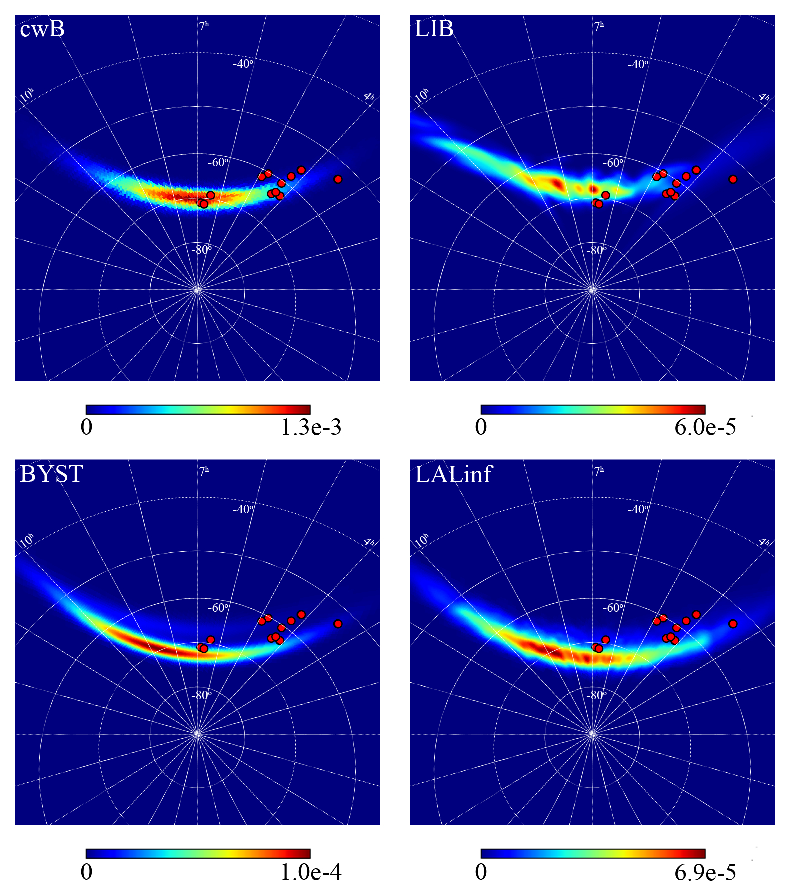
\includegraphics[width=0.5\textwidth]{./slides/plots/src/fig1.pdf}
 % fig1.pdf: 0x0 pixel, 300dpi, 0.00x0.00 cm, bb=
 \caption{The galaxies selected by TOROS collaboration}
 \label{fig:galaxies selected}
\end{figure}

\end{frame}
%%%%%%%%%%%%%%%%%%%%%%%%%%%%%%%%%%%%%%%%%%%%%%%%%%%%%%%%%%%%%%%
\begin{frame}
 We used the Estaci\'on Astrof\'{\i}ca de Bosque Alegre 60 inch (1.54m) telescope. 
 
 \begin{figure}
 \centering
 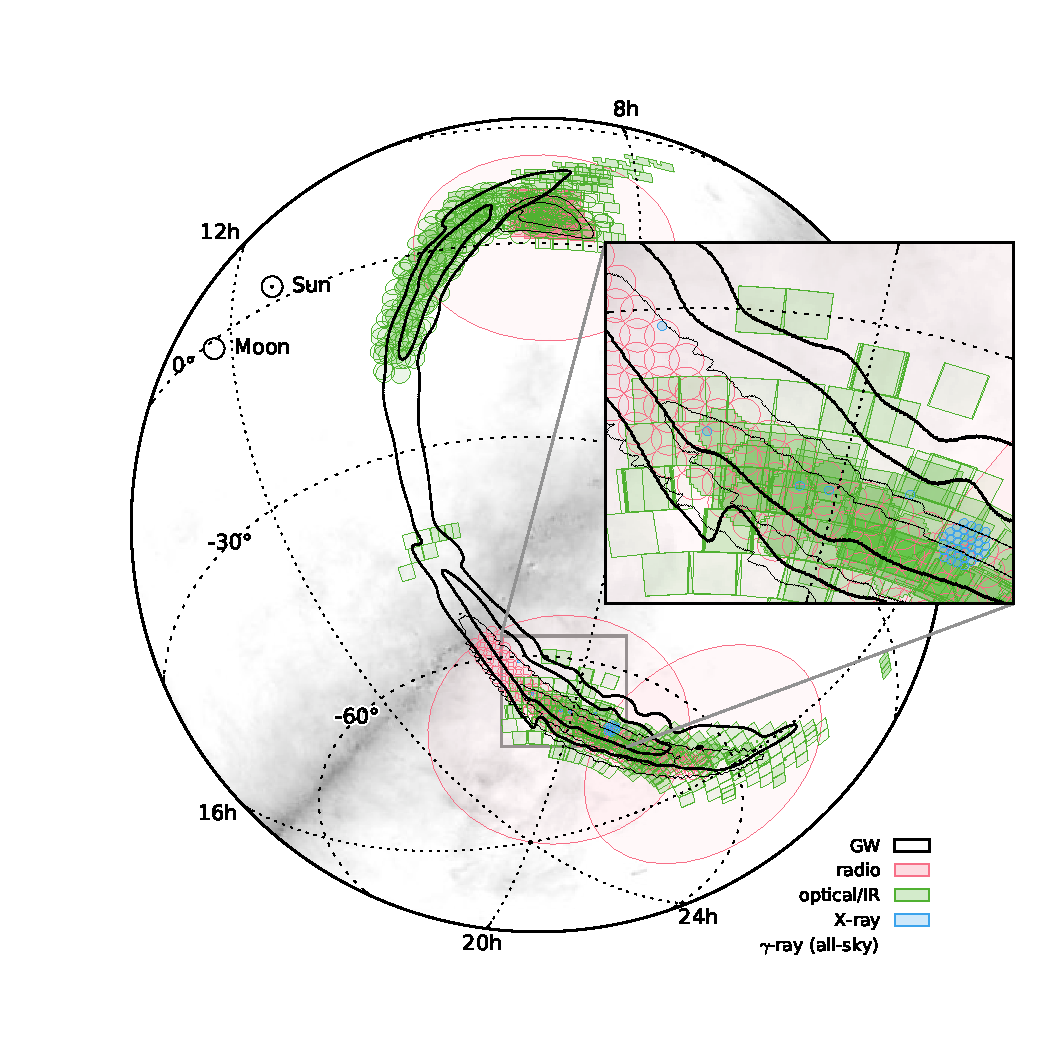
\includegraphics[width=0.7\textwidth]{./slides/plots/160208492v4/tiles.pdf}
 % tiles.pdf: 0x0 pixel, 300dpi, 0.00x0.00 cm, bb=
 \caption{The observation tiles for electromagnetic search.}
 \label{fig:tiles}
\end{figure}

 \end{frame}
%%%%%%%%%%%%%%%%%%%%%%%%%%%%%%%%%%%%%%%%%%%%%%%%%%%%%%%%%%%%%%%
\begin{frame}
 The observations from several collaborations could not find
 a transient associated to this Gravitation Wave event.\\
 
Although we now know that all of them were likely to be CBC.
\begin{figure}
 \centering
 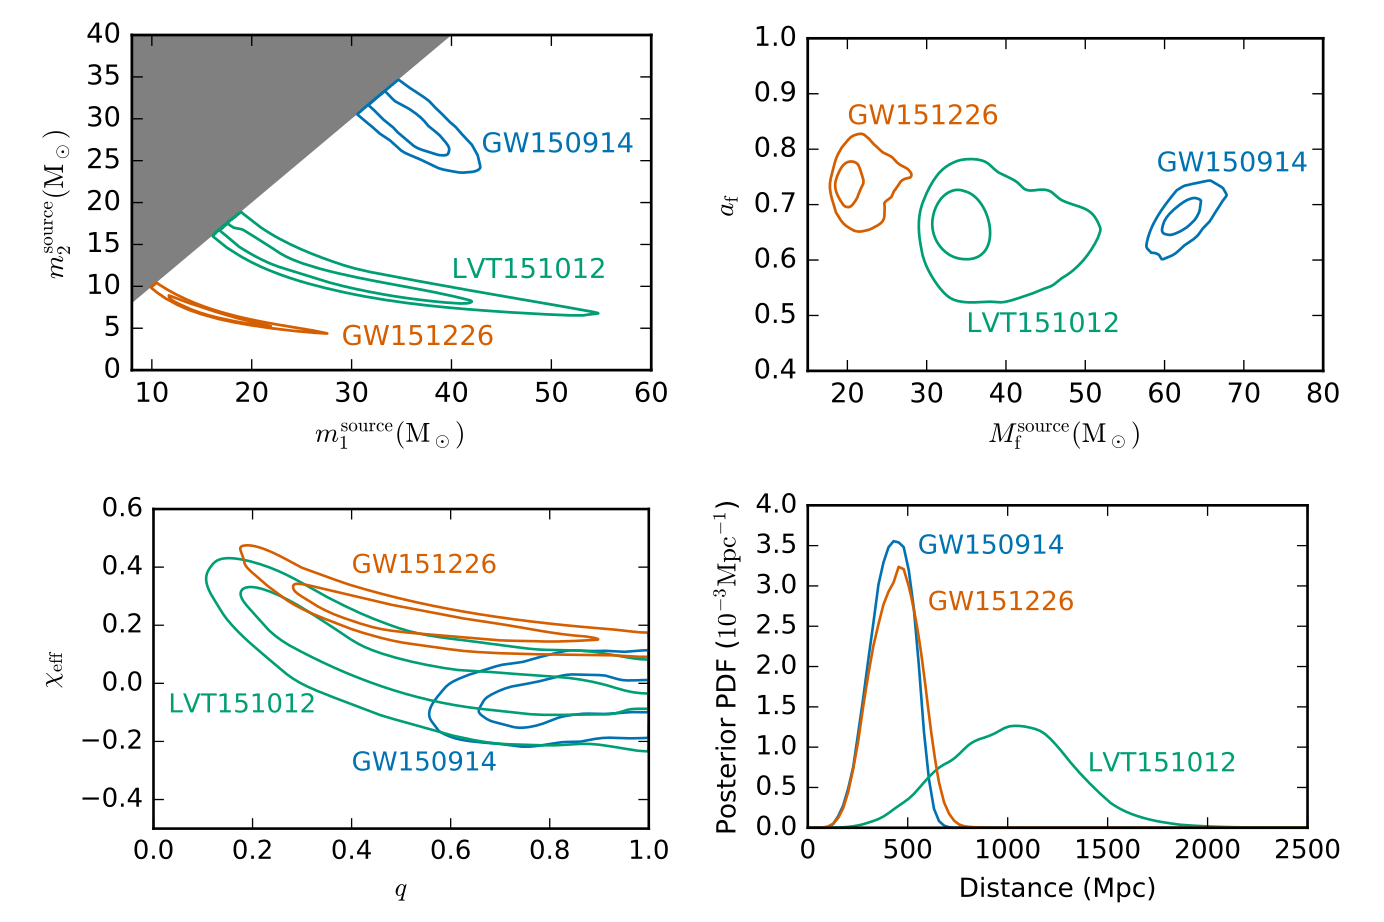
\includegraphics[width=0.75\textwidth]{./slides/plots/posterior_estiamations.png}
 % posterior_estiamations.png: 0x0 pixel, 300dpi, 0.00x0.00 cm, bb=
 \label{fig:posterior}
\end{figure}

\end{frame}

%%%%%%%%%%%%%%%%%%%%%%%%%%%%%%%%%%%%%%%%%%%%%%%%%%%%%%%%%%%%%%%
\begin{frame}
Currently the project is operational in O2 observing run of A-LIGO, but
due to technical issues at the mountain top, we are working on the installation 
of telescopes at lower levels (3400m) in Tolar Grande town.
%\pause
The 2017 campaigns are focusing on new moon, 15 days-long, observation
runs every month. 

\begin{figure}
 \centering
 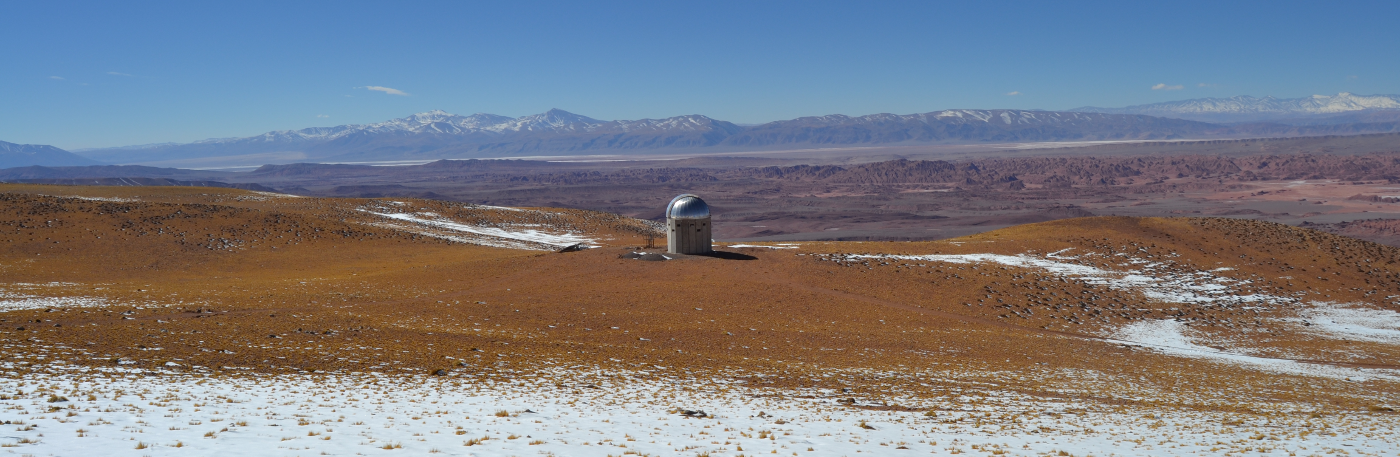
\includegraphics[width=1.\textwidth]{./slides/plots/macon.png}
 % macon.png: 0x0 pixel, 300dpi, 0.00x0.00 cm, bb=
\end{figure}

\end{frame}
%%%%%%%%%%%%%%%%%%%%%%%%%%%%%%%%%%%%%%%%%%%%%%%%%%%%%%%%%%%%%%%
\section{Conclusions and future prospects}
\begin{frame}

\begin{itemize}
\item Our experience in follow ups of GW alarms is greater now, 
we have been following O2 alarms as well.

 \item TOROS now includes several new associated instruments
from Chile (Mamalluca observatory), Texas (at the UTRGV school-telescope)
and Mexico. 

\item In addition we have spectroscopic time in Southern Gemini, and
GTC. 

\item Instruments in Tolar are going to be installed this winter (southern)
with a prospect of continue observation capability.

\end{itemize}

\end{frame}
%%%%%%%%%%%%%%%%%%%%%%%%%%%%%%%%%%%%%%%%%%%%%%%%%%%%%%%%%%%%%%%
\begin{frame}
Thanks! 
\end{frame}



\end{document}
